%% bare_conf_compsoc.tex
%% V1.4b
%% 2015/08/26
%% by Michael Shell
%% See:
%% http://www.michaelshell.org/
%% for current contact information.
%%
%% This is a skeleton file demonstrating the use of IEEEtran.cls
%% (requires IEEEtran.cls version 1.8b or later) with an IEEE Computer
%% Society conference paper.
%%
%% Support sites:
%% http://www.michaelshell.org/tex/ieeetran/
%% http://www.ctan.org/pkg/ieeetran
%% and
%% http://www.ieee.org/

%%*************************************************************************
%% Legal Notice:
%% This code is offered as-is without any warranty either expressed or
%% implied; without even the implied warranty of MERCHANTABILITY or
%% FITNESS FOR A PARTICULAR PURPOSE! 
%% User assumes all risk.
%% In no event shall the IEEE or any contributor to this code be liable for
%% any damages or losses, including, but not limited to, incidental,
%% consequential, or any other damages, resulting from the use or misuse
%% of any information contained here.
%%
%% All comments are the opinions of their respective authors and are not
%% necessarily endorsed by the IEEE.
%%
%% This work is distributed under the LaTeX Project Public License (LPPL)
%% ( http://www.latex-project.org/ ) version 1.3, and may be freely used,
%% distributed and modified. A copy of the LPPL, version 1.3, is included
%% in the base LaTeX documentation of all distributions of LaTeX released
%% 2003/12/01 or later.
%% Retain all contribution notices and credits.
%% ** Modified files should be clearly indicated as such, including  **
%% ** renaming them and changing author support contact information. **
%%*************************************************************************


% *** Authors should verify (and, if needed, correct) their LaTeX system  ***
% *** with the testflow diagnostic prior to trusting their LaTeX platform ***
% *** with production work. The IEEE's font choices and paper sizes can   ***
% *** trigger bugs that do not appear when using other class files.       ***                          ***
% The testflow support page is at:
% http://www.michaelshell.org/tex/testflow/



\documentclass[conference,compsoc]{IEEEtran}
% Some/most Computer Society conferences require the compsoc mode option,
% but others may want the standard conference format.
%
% If IEEEtran.cls has not been installed into the LaTeX system files,
% manually specify the path to it like:
% \documentclass[conference,compsoc]{../sty/IEEEtran}

\usepackage[spanish]{babel}

% Some very useful LaTeX packages include:
% (uncomment the ones you want to load)


% *** MISC UTILITY PACKAGES ***
%
%\usepackage{ifpdf}
% Heiko Oberdiek's ifpdf.sty is very useful if you need conditional
% compilation based on whether the output is pdf or dvi.
% usage:
% \ifpdf
%   % pdf code
% \else
%   % dvi code
% \fi
% The latest version of ifpdf.sty can be obtained from:
% http://www.ctan.org/pkg/ifpdf
% Also, note that IEEEtran.cls V1.7 and later provides a builtin
% \ifCLASSINFOpdf conditional that works the same way.
% When switching from latex to pdflatex and vice-versa, the compiler may
% have to be run twice to clear warning/error messages.






% *** CITATION PACKAGES ***
%
\ifCLASSOPTIONcompsoc
  % IEEE Computer Society needs nocompress option
  % requires cite.sty v4.0 or later (November 2003)
  \usepackage[nocompress]{cite}
\else
  % normal IEEE
  \usepackage{cite}
\fi
% cite.sty was written by Donald Arseneau
% V1.6 and later of IEEEtran pre-defines the format of the cite.sty package
% \cite{} output to follow that of the IEEE. Loading the cite package will
% result in citation numbers being automatically sorted and properly
% "compressed/ranged". e.g., [1], [9], [2], [7], [5], [6] without using
% cite.sty will become [1], [2], [5]--[7], [9] using cite.sty. cite.sty's
% \cite will automatically add leading space, if needed. Use cite.sty's
% noadjust option (cite.sty V3.8 and later) if you want to turn this off
% such as if a citation ever needs to be enclosed in parenthesis.
% cite.sty is already installed on most LaTeX systems. Be sure and use
% version 5.0 (2009-03-20) and later if using hyperref.sty.
% The latest version can be obtained at:
% http://www.ctan.org/pkg/cite
% The documentation is contained in the cite.sty file itself.
%
% Note that some packages require special options to format as the Computer
% Society requires. In particular, Computer Society  papers do not use
% compressed citation ranges as is done in typical IEEE papers
% (e.g., [1]-[4]). Instead, they list every citation separately in order
% (e.g., [1], [2], [3], [4]). To get the latter we need to load the cite
% package with the nocompress option which is supported by cite.sty v4.0
% and later.


%\usepackage{caption}
\usepackage{subcaption}


% *** GRAPHICS RELATED PACKAGES ***
%
\ifCLASSINFOpdf
  \usepackage[pdftex]{graphicx}
  % declare the path(s) where your graphic files are
  % \graphicspath{{../pdf/}{../jpeg/}}
  % and their extensions so you won't have to specify these with
  % every instance of \includegraphics
  % \DeclareGraphicsExtensions{.pdf,.jpeg,.png}
\else
  % or other class option (dvipsone, dvipdf, if not using dvips). graphicx
  % will default to the driver specified in the system graphics.cfg if no
  % driver is specified.
  % \usepackage[dvips]{graphicx}
  % declare the path(s) where your graphic files are
  % \graphicspath{{../eps/}}
  % and their extensions so you won't have to specify these with
  % every instance of \includegraphics
  % \DeclareGraphicsExtensions{.eps}
\fi
% graphicx was written by David Carlisle and Sebastian Rahtz. It is
% required if you want graphics, photos, etc. graphicx.sty is already
% installed on most LaTeX systems. The latest version and documentation
% can be obtained at: 
% http://www.ctan.org/pkg/graphicx
% Another good source of documentation is "Using Imported Graphics in
% LaTeX2e" by Keith Reckdahl which can be found at:
% http://www.ctan.org/pkg/epslatex
%
% latex, and pdflatex in dvi mode, support graphics in encapsulated
% postscript (.eps) format. pdflatex in pdf mode supports graphics
% in .pdf, .jpeg, .png and .mps (metapost) formats. Users should ensure
% that all non-photo figures use a vector format (.eps, .pdf, .mps) and
% not a bitmapped formats (.jpeg, .png). The IEEE frowns on bitmapped formats
% which can result in "jaggedy"/blurry rendering of lines and letters as
% well as large increases in file sizes.
%
% You can find documentation about the pdfTeX application at:
% http://www.tug.org/applications/pdftex





% *** MATH PACKAGES ***
%
%\usepackage{amsmath}
% A popular package from the American Mathematical Society that provides
% many useful and powerful commands for dealing with mathematics.
%
% Note that the amsmath package sets \interdisplaylinepenalty to 10000
% thus preventing page breaks from occurring within multiline equations. Use:
%\interdisplaylinepenalty=2500
% after loading amsmath to restore such page breaks as IEEEtran.cls normally
% does. amsmath.sty is already installed on most LaTeX systems. The latest
% version and documentation can be obtained at:
% http://www.ctan.org/pkg/amsmath





% *** SPECIALIZED LIST PACKAGES ***
%
%\usepackage{algorithmic}
% algorithmic.sty was written by Peter Williams and Rogerio Brito.
% This package provides an algorithmic environment fo describing algorithms.
% You can use the algorithmic environment in-text or within a figure
% environment to provide for a floating algorithm. Do NOT use the algorithm
% floating environment provided by algorithm.sty (by the same authors) or
% algorithm2e.sty (by Christophe Fiorio) as the IEEE does not use dedicated
% algorithm float types and packages that provide these will not provide
% correct IEEE style captions. The latest version and documentation of
% algorithmic.sty can be obtained at:
% http://www.ctan.org/pkg/algorithms
% Also of interest may be the (relatively newer and more customizable)
% algorithmicx.sty package by Szasz Janos:
% http://www.ctan.org/pkg/algorithmicx




% *** ALIGNMENT PACKAGES ***
%
%\usepackage{array}
% Frank Mittelbach's and David Carlisle's array.sty patches and improves
% the standard LaTeX2e array and tabular environments to provide better
% appearance and additional user controls. As the default LaTeX2e table
% generation code is lacking to the point of almost being broken with
% respect to the quality of the end results, all users are strongly
% advised to use an enhanced (at the very least that provided by array.sty)
% set of table tools. array.sty is already installed on most systems. The
% latest version and documentation can be obtained at:
% http://www.ctan.org/pkg/array


% IEEEtran contains the IEEEeqnarray family of commands that can be used to
% generate multiline equations as well as matrices, tables, etc., of high
% quality.




% *** SUBFIGURE PACKAGES ***
%\ifCLASSOPTIONcompsoc
%  \usepackage[caption=false,font=footnotesize,labelfont=sf,textfont=sf]{subfig}
%\else
%  \usepackage[caption=false,font=footnotesize]{subfig}
%\fi
% subfig.sty, written by Steven Douglas Cochran, is the modern replacement
% for subfigure.sty, the latter of which is no longer maintained and is
% incompatible with some LaTeX packages including fixltx2e. However,
% subfig.sty requires and automatically loads Axel Sommerfeldt's caption.sty
% which will override IEEEtran.cls' handling of captions and this will result
% in non-IEEE style figure/table captions. To prevent this problem, be sure
% and invoke subfig.sty's "caption=false" package option (available since
% subfig.sty version 1.3, 2005/06/28) as this is will preserve IEEEtran.cls
% handling of captions.
% Note that the Computer Society format requires a sans serif font rather
% than the serif font used in traditional IEEE formatting and thus the need
% to invoke different subfig.sty package options depending on whether
% compsoc mode has been enabled.
%
% The latest version and documentation of subfig.sty can be obtained at:
% http://www.ctan.org/pkg/subfig



\usepackage{float}
% *** FLOAT PACKAGES ***
%
%\usepackage{fixltx2e}
% fixltx2e, the successor to the earlier fix2col.sty, was written by
% Frank Mittelbach and David Carlisle. This package corrects a few problems
% in the LaTeX2e kernel, the most notable of which is that in current
% LaTeX2e releases, the ordering of single and double column floats is not
% guaranteed to be preserved. Thus, an unpatched LaTeX2e can allow a
% single column figure to be placed prior to an earlier double column
% figure.
% Be aware that LaTeX2e kernels dated 2015 and later have fixltx2e.sty's
% corrections already built into the system in which case a warning will
% be issued if an attempt is made to load fixltx2e.sty as it is no longer
% needed.
% The latest version and documentation can be found at:
% http://www.ctan.org/pkg/fixltx2e


%\usepackage{stfloats}
% stfloats.sty was written by Sigitas Tolusis. This package gives LaTeX2e
% the ability to do double column floats at the bottom of the page as well
% as the top. (e.g., "\begin{figure*}[!b]" is not normally possible in
% LaTeX2e). It also provides a command:
%\fnbelowfloat
% to enable the placement of footnotes below bottom floats (the standard
% LaTeX2e kernel puts them above bottom floats). This is an invasive package
% which rewrites many portions of the LaTeX2e float routines. It may not work
% with other packages that modify the LaTeX2e float routines. The latest
% version and documentation can be obtained at:
% http://www.ctan.org/pkg/stfloats
% Do not use the stfloats baselinefloat ability as the IEEE does not allow
% \baselineskip to stretch. Authors submitting work to the IEEE should note
% that the IEEE rarely uses double column equations and that authors should try
% to avoid such use. Do not be tempted to use the cuted.sty or midfloat.sty
% packages (also by Sigitas Tolusis) as the IEEE does not format its papers in
% such ways.
% Do not attempt to use stfloats with fixltx2e as they are incompatible.
% Instead, use Morten Hogholm'a dblfloatfix which combines the features
% of both fixltx2e and stfloats:
%
% \usepackage{dblfloatfix}
% The latest version can be found at:
% http://www.ctan.org/pkg/dblfloatfix




% *** PDF, URL AND HYPERLINK PACKAGES ***
%
%\usepackage{url}
% url.sty was written by Donald Arseneau. It provides better support for
% handling and breaking URLs. url.sty is already installed on most LaTeX
% systems. The latest version and documentation can be obtained at:
% http://www.ctan.org/pkg/url
% Basically, \url{my_url_here}.




% *** Do not adjust lengths that control margins, column widths, etc. ***
% *** Do not use packages that alter fonts (such as pslatex).         ***
% There should be no need to do such things with IEEEtran.cls V1.6 and later.
% (Unless specifically asked to do so by the journal or conference you plan
% to submit to, of course. )


% correct bad hyphenation here
\hyphenation{op-tical net-works semi-conduc-tor}


\begin{document}
%
% paper title
% Titles are generally capitalized except for words such as a, an, and, as,
% at, but, by, for, in, nor, of, on, or, the, to and up, which are usually
% not capitalized unless they are the first or last word of the title.
% Linebreaks \\ can be used within to get better formatting as desired.
% Do not put math or special symbols in the title.
\title{Segmentación semántica de imágenes}


% author names and affiliations
% use a multiple column layout for up to three different
% affiliations
\author{\IEEEauthorblockN{Francisco Javier Paredes Núñez }
\IEEEauthorblockA{Ingeniero en Informática\\Facultad Politécnica\\Universidad Nacional de Asunción\\
Asunción, Paraguay\\
Email: franciscojavierparedesnunez@fpuna.edu.py}
}

% conference papers do not typically use \thanks and this command
% is locked out in conference mode. If really needed, such as for
% the acknowledgment of grants, issue a \IEEEoverridecommandlockouts
% after \documentclass

% for over three affiliations, or if they all won't fit within the width
% of the page (and note that there is less available width in this regard for
% compsoc conferences compared to traditional conferences), use this
% alternative format:
% 
%\author{\IEEEauthorblockN{Michael Shell\IEEEauthorrefmark{1},
%Homer Simpson\IEEEauthorrefmark{2},
%James Kirk\IEEEauthorrefmark{3}, 
%Montgomery Scott\IEEEauthorrefmark{3} and
%Eldon Tyrell\IEEEauthorrefmark{4}}
%\IEEEauthorblockA{\IEEEauthorrefmark{1}School of Electrical and Computer Engineering\\
%Georgia Institute of Technology,
%Atlanta, Georgia 30332--0250\\ Email: see http://www.michaelshell.org/contact.html}
%\IEEEauthorblockA{\IEEEauthorrefmark{2}Twentieth Century Fox, Springfield, USA\\
%Email: homer@thesimpsons.com}
%\IEEEauthorblockA{\IEEEauthorrefmark{3}Starfleet Academy, San Francisco, California 96678-2391\\
%Telephone: (800) 555--1212, Fax: (888) 555--1212}
%\IEEEauthorblockA{\IEEEauthorrefmark{4}Tyrell Inc., 123 Replicant Street, Los Angeles, California 90210--4321}}




% use for special paper notices
%\IEEEspecialpapernotice{(Invited Paper)}




% make the title area
\maketitle

% As a general rule, do not put math, special symbols or citations
% in the abstract
\begin{abstract}
La segmentación de imagen es un método para aislar un conjunto de áreas de una imagen de acuerdo a ciertas características como color, textura, umbrales, etc. Al realizar esta segmentación se realiza un separado o etiquetado de cada píxel de una imagen, esta división o segmentación agrupa objetos, conjunto de píxeles, con similares características. En ciertas circunstancias es necesario realizar una nueva división sobre estos segmentos similares, como por ejemplo tratar de separar todas las manzanas de una cesta de tal manera a poder contarlos. En la actualidad existen muchas metodologías para la segmentación de imágenes y algunas de ellas enfocadas a la segmentación semántica como las basadas en redes neuronales y algoritmos evolutivos. En este trabajo presentamos algunos de los algoritmos de segmentación.
\end{abstract}

\providecommand{\keywords}[1]{\textbf{\textit{segmentación}}#1}

% no keywords

% For peer review papers, you can put extra information on the cover
% page as needed:
% \ifCLASSOPTIONpeerreview
% \begin{center} \bfseries EDICS Category: 3-BBND \end{center}
% \fi
%
% For peerreview papers, this IEEEtran command inserts a page break and
% creates the second title. It will be ignored for other modes.
\IEEEpeerreviewmaketitle



\section{Introducción}
% no \IEEEPARstart
La segmentación de imágenes es un proceso en el cual se desea agrupar un conjunto de píxeles de una imagen de acuerdo a ciertas características de la misma \cite{tecsegm}, estas características pueden ser, color, textura, umbral, forma, entre otros, en la figura \ref{fig:setmentacionporcolor} podemos observar una segmentación basada en el color rojo mientras que en la figura \ref{fig:setmentacionporforma} observamos una segmentación basada en la forma cuadrada. La segmentación ha cobrado mucho interés en los últimos tiempos ya que el mismo es utilizado en varios ámbitos como la navegación de robots, diagnósticos médicos, detección de objetos en el espacio y muchas otras. En ciertas circunstancias la segmentación requiere que sea más eficaz y/o eficiente por lo cual se implementan nuevas metodologías para poder lograrlos \cite{segconv}\cite{algen}.

Cuando realizamos la segmentación, es decir, separamos las zonas de interés, en ciertas ocasiones esto no es suficiente, por ejemplo si tenemos una imagen de una cesta de frutas en las cuales existen numerosas manzanas y si quisiéramos contar cuantas manzanas hay en dicha cesta, no solo es suficiente realizar una segmentación de todas las manzanas sino que también es necesario separar por cada manzana, este proceso se conoce como segmentación semántica\cite{segsem}, no todas las metodologías de segmentación pueden realizar esto por lo cual estaremos viendo algunas de las metodologías existentes especificando el por que si o no podría ser utilizado para realizar la segmentación semántica.

Tomaremos especial enfoque a la segmentación semántica basadas redes neuronales convolucionales y algoritmos genéticos ya que estas proveen resultados muy buenos para este tipo de tarea\cite{segconv} y finalizaremos hablando de cómo los algoritmos evolutivos encajan en esta tarea.

%Independientemente de lo mencionado anteriormente se pueden identificar dos propiedades principales por la que se pueden realizar la segmentación.

\begin{figure}[b]
\centering
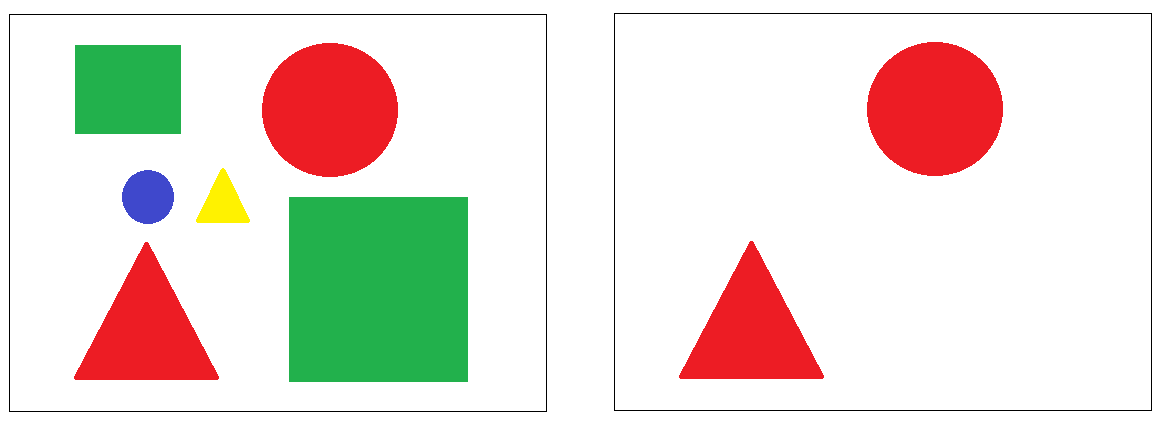
\includegraphics[width=0.4\textwidth]{setmentacionporcolor.png}
\caption{\label{fig:setmentacionporcolor}Segmentación por color: a la derecha tenemos una imagen con muchos objetos y a la derecha una imagen segmentada usando el color rojo.}
\end{figure}

\begin{figure}[h]
\centering
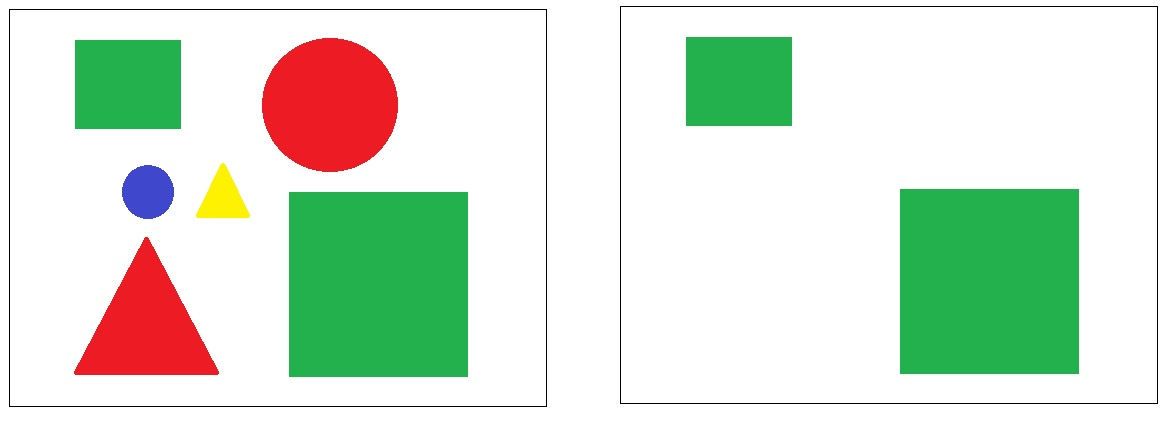
\includegraphics[width=0.4\textwidth]{setmentacionporforma.jpg}
\caption{\label{fig:setmentacionporforma}Segmentación por forma: a la derecha tenemos una imagen con muchos objetos y a la derecha una imagen segmentada usando la forma cuadrada de los objetos.}
\end{figure}

% You must have at least 2 lines in the paragraph with the drop letter
% (should never be an issue)

\section{Segmentación}
Como se ha mencionado la segmentación de imágenes es un proceso para obtener o separar áreas de una imagen, para realizar esta tarea es necesario tener en cuentas las características de la imagen y así obtener las áreas deseadas. En la literatura se han propuesto muchas técnicas de segmentación y cada una con características diferentes sin embargo la mayoría de ellas caen dentro de dos técnicas que se especifican a continuación.

\subsection{Técnicas de segmentación}
Existen numerosas técnicas que pueden ser aplicadas pero una sola no puede ser aplicada para solucionar todos los problemas existentes, es decir, para ciertas circunstancias o necesidades una técnica podría ser mucho más efectiva que otra, es más, en algunas de ellas puede que no sea factible aplicarlas\cite{tecsegm} por ejemplo, las redes neuronales convolucionales son muy buenas pero como ya veremos esta requiere de un entrenamiento que en ciertas circunstancias esto no pueden ser llevado a cabo ya sea por temas de recursos de procesamiento o por falta de imágenes de entrenamiento. 

Estas son las técnicas más utilizadas para realizar la segmentación:

\begin{itemize}
\item \textbf{Detección de discontinuidades:} aquí se intenta detectar los cambios bruscos de colores, entre los algoritmos que implementa esta técnica podemos mencionar la detección de bordes.
\item \textbf{Detección de similitudes:} aquí se definen ciertas características y mediante algún proceso se procede a realizar el filtro de las regiones que poseen las características deseadas, entre los algoritmos que utilizan esta técnica podemos mencionar el método de umbralización (thresholding).
\end{itemize}

\subsection{Algoritmos de segmentación}
A continuación, mostramos algunos de las principales metodologías utilizadas para realizar el trabajo de segmentar las imágenes.

\subsubsection{Segmentación basada en detección de bordes}
Con esta metodología se intenta encontrar los bordes de cada objeto atendiendo los cambios bruscos de una imagen, esta suposición de cambios bruscos como detección de bordes no siempre son correctos especialmente para objetos irregulares. En la figura \ref{fig:bordes} podemos observar una imagen sobre la cual se realiza una segmentación basada en esta técnica.

\begin{figure}[H]
\centering
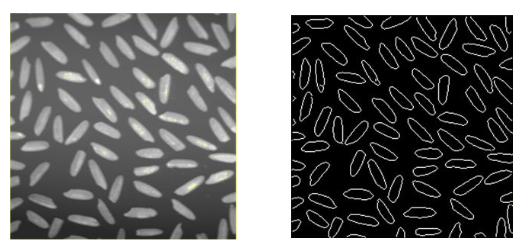
\includegraphics[scale=0.5]{bordes.png}
\caption{\label{fig:bordes}Segmentación basada en bordes}
\end{figure}

\subsubsection{Segmentación basada en histograma}
Con este algoritmo, lo primero que se realiza es transformar la imagen a color a escala de grises, posteriormente calcular su histograma, al obtener este valor se realiza un filtrado sobre la imagen de tal manera que solo queden aquellos que están por encima del un punto elegido del histograma, se verifica que esta metodología posee dos problemas importantes:
\begin{itemize}
    \item El primer problema es identificar cual es el nivel de tono de gris o punto sobre la cual se utilizara para realizar el filtrado.
    \item El segundo problema es que para múltiples objetos que tengan las mismas intensidades de luz será imposible identificar los bordes y por consiguiente separar los objetos para poder contarlos.
\end{itemize}
Como se puede observar en la figura \ref{fig:histograma} se realiza el cálculo del histograma y se selecciona un punto del mismo para realizar el filtrado de la imagen.

\begin{figure}[H]
\centering
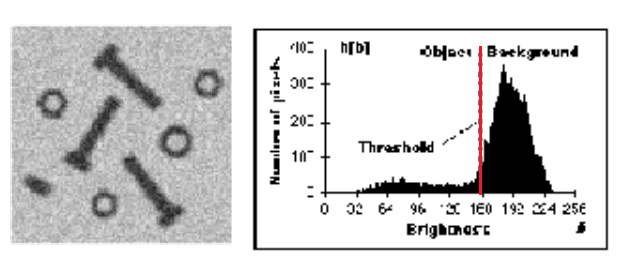
\includegraphics[scale=0.5]{histograma.png}
\caption{\label{fig:histograma}Segmentación basada en histograma}
\end{figure}

\subsubsection{Técnica de gradiente}
Esta técnica está basada en un artificio matemático de derivadas de primer orden en el cual se establece una función f(x,y), el gradiente de una imagen es una convolución y se define como g(f(x,y)), las derivadas de primer orden permiten encontrar los lugares en los cuales la intensidad cambia abruptamente.

El gradiente de una imagen es una función f(x, y) que se define como el vector bidimensional presentado en la siguiente ecuación.

\begin{figure}[H]
\centering
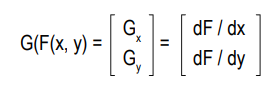
\includegraphics[scale=0.7]{ecgradiente.png}
\end{figure}

El operador gradiente G alcanza su máximo valor en la dirección en que la variación es máxima, en este caso las derivadas de primer orden permiten encontrar lugares en una imagen en donde la intensidad cambia rápidamente y es mayor en magnitud a un umbral especificado. 

De manera similar a la técnica de histograma, este método también es sensible a los ruidos de la imagen, zonas con muchos brillos pueden generar bordes falsos, por esta razón es complicada la segmentación semántica de una imagen.

\subsubsection{Método de crecimiento por región}
Esta metodología se basa en seleccionar un conjunto de puntos dentro de la imagen, estos puntos son conocidos también como semillas, por cada semilla existente, esta se extiende o crece a las zonas (píxeles) aledañas. Para poder crecer o extenderse se deben definir ciertas características por ejemplos, si el vecino adyacente se encuentra dentro de un umbral definido, es importante mencionar que se pueden definir varias características para ir creciendo.

Esta técnica provee buenos resultados, pero tiene un problema, se deben definir las semillas, esto conlleva a preguntas interesantes como, ¿Cuantas semillas son necesarias? ¿Cuál o cuáles son las características necesarias para realizar el crecimiento? ¿Dónde sembrar estas semillas? Aquí una vez más podrían darse problemas en la detección de objetos similares (características similares) para poder realizar la segmentación semántica ya que al definir características similares estas no pueden saber si están correspondiendo al mismo objeto o no.

En la figura \ref{fig:crecimiento} se observa que se selecciona un punto de la imagen, semilla, y a partir de este punto el mismo va creciendo o extendiéndose a los píxeles adyacentes que cumplen ciertas características.

\begin{figure}[H]
\centering
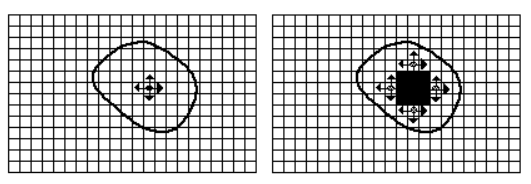
\includegraphics[scale=0.5]{crecimiento.png}
\caption{\label{fig:crecimiento}segmentación por crecimiento}
\end{figure}

\subsubsection{Redes neuronales convolucionales}
Al escuchar redes neuronales convolucionales, Convolutional Neural Network (CNN), pareciera ser algo intimidante sin embargo como lo veremos la idea detrás es bastante simple, esta técnica ha arrojado muy buenos resultados comparando con las anteriores metodologías utilizadas \cite{segconv}. A diferencia de las demás metodologías mencionadas anteriormente entraremos en detalle atendiendo la eficacia de la misma.

La idea principal de con las CNN, es poder extraer las características que definen los componentes u objetos/instancias de una imagen, como se puede apreciar en la figura \ref{fig:formasdesegmentacion}, para poder extraer estas características el proceso debe pasar por un proceso de aprendizaje, este aprendizaje consiste en analizar una serie de imágenes, imágenes de entrenamiento también conocidas conocidas como dataset, es de notar aquí que esto podría ser una desventaja en comparación con las demás metodologías ya que se necesita un preprocesamiento sobre este dataset, este preprocesamiento puede consumir bastante recursos adicionales, entre estos recursos están los recursos computacionales pero, gracias al avance de las tecnologías estos son bastantes accesibles, entonces teniendo de cuenta esto el único problema es el dataset.

\begin{figure}[H]
\centering
\begin{subfigure}{.3\linewidth}
\centering
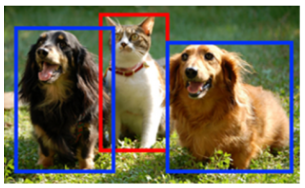
\includegraphics[width = \linewidth]{reconocimiento}
\caption{Reconocimiento de los objetos}
\end{subfigure}%
\hspace{1em}% Space between image A and B
\begin{subfigure}{.3\linewidth}
\centering
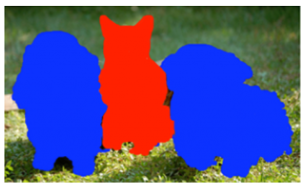
\includegraphics[width = \linewidth]{setmentacionsemantica}
\caption{Segmentación semántica}
\end{subfigure}%
\hspace{2em}% Space between image B and C
\begin{subfigure}{.3\linewidth}
\centering
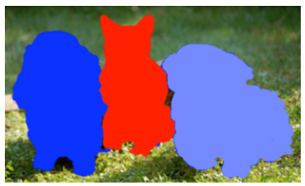
\includegraphics[width = \linewidth]{segmetaciondeinstancias}
\caption{Segmentación de instancias}
\end{subfigure}
\caption{\label{fig:formasdesegmentacion}Segmentación de imágenes}
\end{figure}


En la figura \ref{fig:cnn} se observa una arquitectura CNN utilizada normalmente, se observa una imagen de entrada sobre la cual se aplica una serie de convoluciones que intenta extraer las características. Si aplicamos una CNN sobre la imagen de entrada el mismo debería clasificar todos los píxeles y si agregamos una serie de capas a nuestra red neural y que en cada capa cada neurona esté conectada a todas las neuronas esto sería muy grande y consumiría bastante recursos informáticos, es por esto que se desea obtener las características ya que estos datos son muchos menores a la entrada inicial y por consiguiente al aplicar una conexión completa entre cada capa el mismo no consumiría mucho menos recursos. Se puede observar en la figura \ref{fig:cnn} en cada etapa de convolución y pooling la imagen inicial va disminuyendo y es factible aplicar una red neuronal en la cual todas las neuronas este conectadas a las demás.

\begin{figure}[H]
\centering
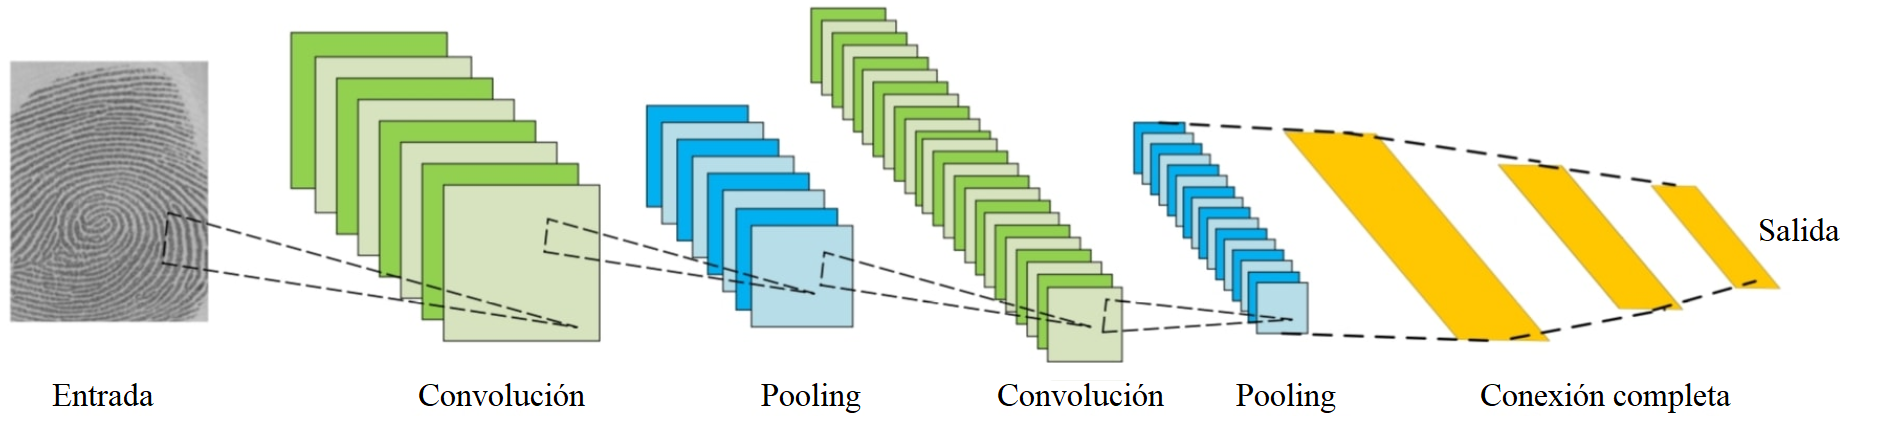
\includegraphics[width=0.4\textwidth]{cnn.png}
\caption{\label{fig:cnn}Arquitectura básica de un red convolucional}
\end{figure}


Una mejora en los CNN tradicionales es la convolución dilatada, la idea aquí es meter agujeros en el kernel de tal manera a obtener resoluciones más grandes y obtener mejores características, esta metodología se aplica a una amplia variedad de tareas como la detección de objetos, flujo óptico y generación de audio\cite{segconv}

Como se ha mencionado la segmentación semántica trata de obtener los objetos o instancias de una imagen, para poder lograrlo debe categorizar o etiquetar cada píxel y las redes neuronales convolucionales presentan un buen rendimiento para realizar esta tarea.

Analizando el estado de arte, actualmente, la segmentación de imágenes tiene tres componentes claves:
\begin{itemize}
  \item Una red convolucional completa (FCN) que se encarga del aprendizaje y la inferencia.
  \item Una CRF (Conditional Random Field) para capturar las dependencias dentro de una imagen para mejorar las predicciones.
  \item Por ultimo, una convolución dilatada, de esto lo hablaremos detalladamente más adelante, pero lo que intenta hacer es aumentar la resolución de ciertas características de tal manera a poder obtener mejores predicciones manteniendo un costo computacional.
\end{itemize}

La idea es mejorar las codificaciones y decodificaciones, es decir el entrenamiento y la manera de obtener la segmentación semántica de las imágenes. Por lo cual se propone un método conocido como Dense Upsampling Convolution (DUC), el cual es bastante sencillo, en vez de tratar de recuperar todos los píxeles de una imagen se aplica un conjunto de filtros aprendidos para aumentar el tamaño de las características reducidas en el proceso de convolución de tal manera a mantener la resolución, esto se logra agregando agujeros en el kernel.

Adicionalmente se propone un cambio el cual es conocido como Hybrid Dilation Convolution (HDC), este cambio realiza lo siguiente, en vez de utilizar el mismo dilatador (kernel con agujeros), se utiliza una concatenación serializada de dilatadores, es decir un conjunto de bloques.

Entonces, para resumir, se utilizan el DUC y HDC para realizar las operaciones convolucionales para obtener una segmentación más eficaz y eficiente, esta arquitectura se puede observar en la imagen \ref{fig:fcn}.

\begin{figure}[H]
\centering
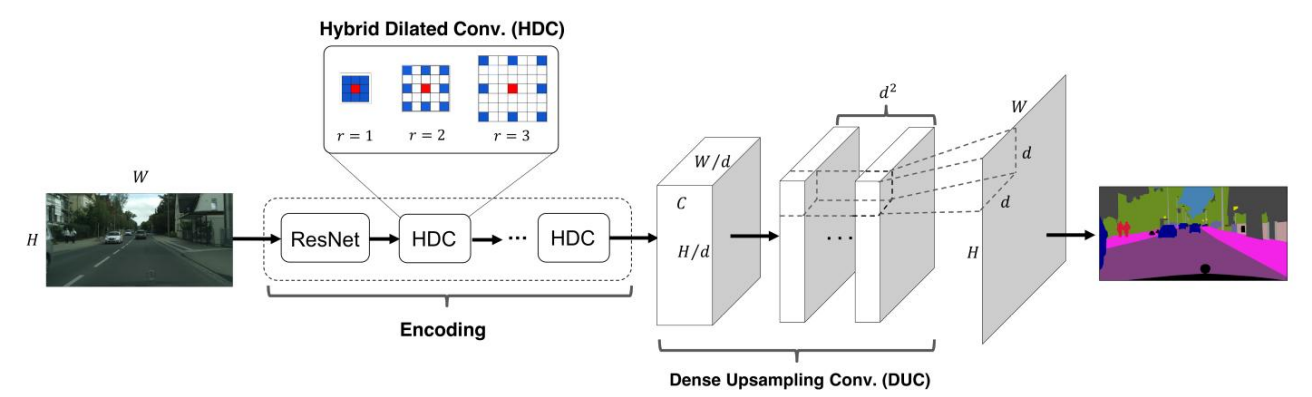
\includegraphics[width=0.5\textwidth]{fcn.png}
\caption{\label{fig:fcn}Arquitectura utilizando HDC y DUC}
\end{figure}

Para comprender mejor DCU, supongamos que una imagen de entrada tiene una altura H, una anchura W y canales de color C, y el objetivo de la segmentación semántica a nivel de píxel es generar un mapa de etiquetas con un tamaño H × W donde cada píxel se etiqueta con una etiqueta de una categoría. Después de introducir la imagen en un FCN, se obtiene un mapa de características con dimensión h × w × c en la capa final antes de hacer predicciones, donde h = H/d, w = W/d y d es el factor de reducción de muestreo.

La convolución dilatada, como se ha mencionado, es utilizada para mantener una alta resolución de los mapas de características en FCN reemplazando la operación de agrupación máxima o la capa de convolución estriada mientras se mantiene el campo receptivo de la capa correspondiente.

La convolución dilatada generalmente se aplica en mapas de características que ya están muestreados para lograr una compensación razonable de eficiencia/precisión.
Sin embargo, existe un problema teórico en el marco de convolución dilatada, se pierde una gran parte (al menos el 75 \%) de la información\cite{segconv}.

Para solucionar este problema los autores del trabajo\cite{segconv} proponen una convolución dilatada híbrida de solución simple (HDC) para abordar este problema teórico. Se propone lo siguiente, en lugar de usar la misma tasa de dilatación para todas las capas después de que se produce la reducción, se utiliza una tasa de dilatación diferente para cada capa.

Lo que se logra con esto es que la capa superior puede acceder a la información de una gama más amplia de píxeles, en la misma región que la configuración original como se puede observar en la figura \ref{fig:condensacion}.

\begin{figure}[H]
\centering
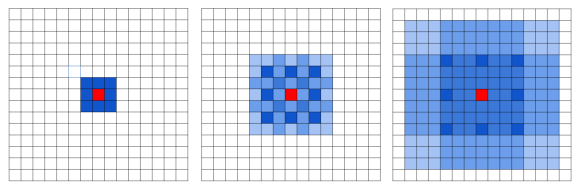
\includegraphics[scale=0.5]{condensacion.png}
\caption{\label{fig:condensacion}Aplicación del kernel dilatado}
\end{figure}
Este proceso se repite en todas las capas, lo que hace que el campo receptivo no cambie en la capa superior, también es importante mencionar que HDC se integra naturalmente con las capas originales de la red, sin necesidad de agregar módulos adicionales.

La arquitectura y la implementación son bastante sencillas y la segmentación resultante es muy buena, existen deferentes mejoraras y avances sobre las redes neuronales sin embargo con lo expuesto anteriormente se logran buenos resultadas.

%Los resultados que se han obtenido sobre tres conjuntos de datos de segmentación semántica: paisajes urbanos, conjunto de datos KITTI para estimación de carreteras y por ultimo sobre PASCAL VOC2012. Se utilizaron redes ResNet-101 y ResNet-152 que fueron entrenado previamente en el conjunto de datos de ImageNet. La capa de salida contiene la cantidad de categorías semánticas que se clasificaron según el conjunto de datos (incluido el fondo, si corresponde). Se utilizó MXNet para entrenar y evaluar todos nuestros modelos.


\subsubsection{Segmentación basada en algoritmos genéticos (AG)}
Los algoritmos genéticos (AG) son una familia de métodos de búsqueda adaptativos que están inspiradas en el proceso evolutivo genético. Una característica importante de esta metodología es su alta eficiencia para encontrar soluciones a problemas en las que se debe realizar búsquedas combinatorias sin quedar atrapados en extremos locales a través de su exploración en un espacio de búsqueda. Por lo tanto, se han convertido en una poderosa alternativa a los métodos de optimización convencionales\cite{algen}. Los AG se han utilizado para la segmentación de imágenes en el pasado, se han aplicado para modificar las funciones de etiquetado, la evaluación de la aptitud se basó en la homogeneidad y especificidad de la región, también se realizaron una investigación sobre la segmentación adaptativa de imágenes utilizando métodos de búsqueda híbridos y genéticos.

En\cite{algen} se presenta un trabajo para la detección de malas hierbas utilizando AG en condiciones de iluminación natural variable, sin embargo, es interesante mencionar que algunos métodos de segmentación de imágenes de vegetación se han basado en el análisis de conglomerados. El problema de la segmentación basada en el análisis de conglomerados es que es sensible a las condiciones de iluminación, la elección de las semillas del conglomerado y la cantidad de conglomerados. Por ejemplo, si se cambiasen las composiciones de diferentes partes de la imagen de diferentes condiciones de iluminación, el resultado de la agrupación sería diferente. Por lo tanto, es complicado crear un mapa de conglomerados universal para detectar de manera sólida la maleza en condiciones de iluminación variables.

En los enfoques basados en el análisis de conglomerados, el análisis de conglomerados se utiliza primero para dividir los datos de la imagen de acuerdo con las similitudes de color. Después de que las regiones de la planta se etiquetan como tales mediante inspección visual, se entrena y utiliza un clasificador Bayes para generar una tabla de búsqueda (LUT) que se emplea durante la segmentación en tiempo real.

Uno de los problemas detectados en el proceso de agrupamiento es que no tiene en cuenta las interacciones espaciales entre los píxeles vecinos y da como resultado una calidad de segmentación más baja.

Lo que se propuso en\cite{algen} fue buscar una región de color relativamente estable en el espacio de color HSI para segmentar la vegetación bajo dos condiciones extremas de iluminación de campo al aire libre como resultado de condiciones de cielo nublado y soleado. Esta región de color podría utilizarse para distinguir las malas hierbas en una gran variedad de condiciones de iluminación.

En la figura \ref{fig:genmosaico} se puede observar cómo se generaron las imágenes, en la izquierda se puede ver una foto obtenida en condiciones de iluminación soleada y con baja densidad de vegetación, en la derecha se puede ver una imagen obtenida en condiciones de iluminación nublada con alta densidad de vegetación. La idea de unir estas imágenes en mosaico con diferentes condiciones de iluminación es la de determinar si el AG puede manejar la variación de iluminación y ubicar una región de color en el espacio HSI y poder utilizar esto para posteriormente realizar la segmentación.

\begin{figure}[H]
\centering
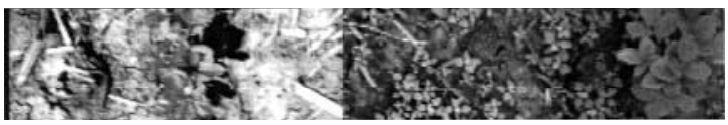
\includegraphics[scale=0.5]{genmosaico.png}
\caption{\label{fig:genmosaico}Parte de la imagen generada}
\end{figure}
 
Una vez realizada la segmentación se debe realizar la comparación o verificación de la calidad del mismo por lo cual se hicieron segmentaciones de imágenes de manera manual para posteriormente verificar píxel por píxel la precisión de la segmentación realizada por el AG, la segmentación manual fue realizada por humanos pintando los píxeles de la planta en las imágenes con un color común.
 
Una importante características del cual debemos hablar es el espacio de colores que es utilizado por el AG para realizar la segmentación, se observa que la intensidad domina la dispersión en los datos de los píxeles en el espacio RGB (rojo, verde y azul) con puntos de datos que forman regiones en forma de cigarro a lo largo del eje de intensidad como se puede observar en la figura \ref{fig:cigarro}. En este tipo de distribución no se observa a simple vista los métodos simples de umbralización del tipo límite mínimo-máximo. Además, las coordenadas RGB no normalizadas podrían variar mucho según las condiciones de la imagen.

\begin{figure}[H]
\centering
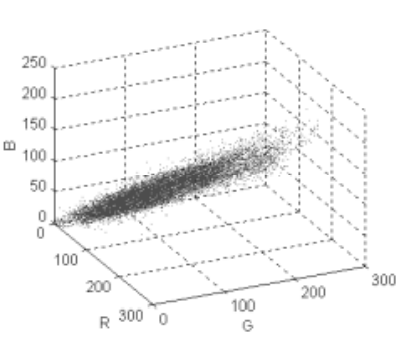
\includegraphics[scale=0.5]{cigarro.png}
\caption{\label{fig:cigarro}Distribución de colores RGB}
\end{figure}

Con respecto a las coordenadas RGB normalizadas, es decir, las coordenadas de cromaticidad forman el triángulo de color, que define los componentes de color (tono y saturación) del modelo HSI. Además, el tono, la saturación y la intensidad son características generales que se utilizan para distinguir un color de otro. HUE representa la longitud de onda dominante en una mezcla de ondas de luz y, por lo tanto, es el carácter dominante. La saturación es la pureza relativa o la cantidad de luz blanca mezclada con un matiz; por lo tanto, los colores del espectro puro están completamente saturados.

El tono y la saturación considerados juntos se denominan cromaticidad; por tanto, un color puede caracterizarse por su intensidad y cromaticidad. El modelo HSI desacopla el componente de intensidad de la información de color, y los componentes de tono y saturación están relacionados con la forma en que los seres humanos perciben el color. Por lo tanto, el modelo HSI es una herramienta ideal para desarrollar algoritmos de procesamiento de imágenes basados en algunas de las propiedades de detección de color del sistema visual humano.

En \cite{algen} se hace la suposición de que existe una región cuboide que define todos los píxeles de las plantas, porque los píxeles de las plantas deberían ser "verdes" con diferentes niveles de saturación e intensidad. Sin embargo, el fondo debe ser la región de los píxeles "grises", que consta de suelo, roca y residuos.

Esta suposición es algo limitante con respecto a realizar la segmentación de imágenes que tengan varios colores sin embargo hay que recordar que se quiere detectar solo la maleza en este trabajo.

\paragraph\textbf{Diseño del AG}

La característica principal del AG radica en su capacidad para explotar la información acumulada de un dominio inicialmente desconocido de una manera altamente eficiente, por esta razón, los autores \cite{algen} utilizaron el AG para diseñar un motor de búsqueda en esta investigación.

\paragraph\textbf{Componentes y operadores del AG}

\textbf{Cromosoma:} El cromosoma está formada por una cadena binaria de 48 bits, un cromosoma, representaba los límites de la región de la planta en el espacio HSI. A cada parámetro límite se le asignó una ubicación fija de un byte de longitud en el cromosoma.

Con base en el conocimiento de la definición del espacio de color HSI y el objetivo de detección de malas hierbas, la cadena se organizó con el límite de tono superior como el primer byte en el cromosoma seguido por el límite de tono inferior, ya que el tono es la característica de color más destacada. Los siguientes dos bytes fueron los límites de saturación superior e inferior. Los límites de intensidad fueron los últimos dos bytes ya que la intensidad es independiente del color y por lo tanto de menor importancia. En la figura \ref{fig:cromosoma} se puede observar cómo está distribuida o conformada un cromosoma.

\begin{figure}[H]
\centering
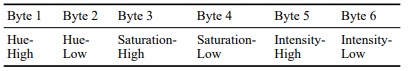
\includegraphics[scale=1]{cromosoma.png}
\caption{\label{fig:cromosoma}Cromosoma}
\end{figure}

\textbf{Tamaño de la población:} Los elementos básicos de un AG se denominan estructuras de conocimiento o individuos. A un conjunto de individuos se le llama población. La regla empírica \cite{goldberg} exige un tamaño de población aproximadamente igual a la longitud del cromosoma. En este trabajo la longitud de un cromosoma es de 48 bits por lo cual se utilizó un tamaño de 48 individuos.

\textbf{Selección:} Para la selección de individuo se implementó la selección de torneos locales sin reemplazo. La selección de torneos locales, que selecciona al individuo con la mejor evaluación entre individuos elegidos al azar.

\textbf{Cruce y Mutación:} El cruce y la mutación determinan la composición genética de la descendencia a partir del material genético de los padres. Se utilizó un punto de cruce único entre los cromosomas seleccionados para generar una nueva población para cada generación. También se eligió un valor de probabilidad de cruce de 0,8. La mutación proporciona cambios ocasionales en la operación de cruzamiento al invertir uno o más elementos genéticos durante la reproducción de tal manera a poder expandir el espacio de búsqueda. 

\textbf{Restricciones:} Los límites superiores deben ser más grandes que sus límites inferiores correspondientes, durante el proceso de cruzamiento y mutación estas reglas pueden incumplirse por lo cual se realiza unos ajustes al mismo.

\textbf{Evaluación de funciones:} Para realizar la evaluación se analiza la segmentación de la imagen. Se toman en cuenta los siguientes datos, la sensibilidad al objeto (SenO) y la sensibilidad al fondo (SenB). SenO es la relación entre los píxeles de plantas correctamente segmentados en la imagen de prueba y el número total de píxeles de plantas en la imagen de referencia. SenB es la relación entre el número de píxeles de fondo segmentados correctamente en la imagen de prueba y el número total de píxeles de fondo en la figura \ref{fig:diagben} de referencia.

\begin{figure}[H]
\centering
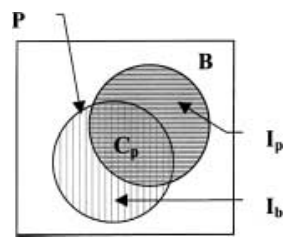
\includegraphics[scale=0.5]{diagben.png}
\caption{\label{fig:diagben}Figura 4: Diagrama de Venn que muestra los conjuntos de píxeles segmentados en la imagen de referencia y la imagen de prueba, respectivamente. P y B son los conjuntos de píxeles de planta y fondo en la imagen de referencia, respectivamente. CP es el conjunto de píxeles de plantas correctamente segmentados en la imagen de prueba. Ip e Ib son los conjuntos de píxeles incorrectamente segmentados como planta y fondo, respectivamente.}
\end{figure}

\textbf{Criterios de parada:} Un aspecto importante del algoritmo es saber cuándo detenerse, para este trabajo el algoritmo se detiene si cumple algunas de las tres condiciones siguientes:

\begin{itemize}
  \item si se localiza un conjunto de parámetros utópicos, como por ejemplo si el valor de aptitud se encuentra por encima de un umbral de aceptación predefinido (99\%).
  \item si la mejor aptitud de las poblaciones no mejoraba durante cinco generaciones consecutivas.
  \item si el número de generación era superior a 100.
\end{itemize}

\paragraph\textbf{Evaluación de método propuesto para la segmentación} 

Para medir el rendimiento de la segmentación de este trabajo, se segmentó el mismo conjunto de imágenes utilizado por\cite{steward}. Las medidas de rendimiento utilizadas para su investigación y descritas anteriormente se calcularon y compararon con las informadas en su trabajo sobre investigación de segmentación de imágenes basada en agrupamiento y transformación de color.

\paragraph \textbf{Resultados} 

La aptitud de 0,9003 fue el mejor valor logrado con la función FB para todos los tamaños de población menores de 100 generaciones, existe la posibilidad de que un modelo AG avanzado (AG desordenado) podría mejorar aún más el rendimiento de este trabajo. Un método desordenado de AG es usar "operadores aumentados por conocimiento" para el cruce. Por ejemplo, el cruce multipunto en los bordes de los límites puede conducir a un mejor rendimiento.

Los resultados generales de la segmentación fueron buenos tanto en las partes de la imagen soleadas como en las nubladas por lo cual el proceso de segmentación en el dominio HSI mostró claramente que encontró esos píxeles de tono vegetal verdoso dentro de un cierto rango de saturación e intensidad.
Este resultado implica que existe una región en el espacio de color HSI donde existe la mayoría de los píxeles de la planta independientemente de la variación en las condiciones de iluminación. 


% An example of a floating figure using the graphicx package.
% Note that \label must occur AFTER (or within) \caption.
% For figures, \caption should occur after the \includegraphics.
% Note that IEEEtran v1.7 and later has special internal code that
% is designed to preserve the operation of \label within \caption
% even when the captionsoff option is in effect. However, because
% of issues like this, it may be the safest practice to put all your
% \label just after \caption rather than within \caption{}.
%
% Reminder: the "draftcls" or "draftclsnofoot", not "draft", class
% option should be used if it is desired that the figures are to be
% displayed while in draft mode.
%
%\begin{figure}[!t]
%\centering
%\includegraphics[width=2.5in]{myfigure}
% where an .eps filename suffix will be assumed under latex, 
% and a .pdf suffix will be assumed for pdflatex; or what has been declared
% via \DeclareGraphicsExtensions.
%\caption{Simulation results for the network.}
%\label{fig_sim}
%\end{figure}

% Note that the IEEE typically puts floats only at the top, even when this
% results in a large percentage of a column being occupied by floats.


% An example of a double column floating figure using two subfigures.
% (The subfig.sty package must be loaded for this to work.)
% The subfigure \label commands are set within each subfloat command,
% and the \label for the overall figure must come after \caption.
% \hfil is used as a separator to get equal spacing.
% Watch out that the combined width of all the subfigures on a 
% line do not exceed the text width or a line break will occur.
%
%\begin{figure*}[!t]
%\centering
%\subfloat[Case I]{\includegraphics[width=2.5in]{box}%
%\label{fig_first_case}}
%\hfil
%\subfloat[Case II]{\includegraphics[width=2.5in]{box}%
%\label{fig_second_case}}
%\caption{Simulation results for the network.}
%\label{fig_sim}
%\end{figure*}
%
% Note that often IEEE papers with subfigures do not employ subfigure
% captions (using the optional argument to \subfloat[]), but instead will
% reference/describe all of them (a), (b), etc., within the main caption.
% Be aware that for subfig.sty to generate the (a), (b), etc., subfigure
% labels, the optional argument to \subfloat must be present. If a
% subcaption is not desired, just leave its contents blank,
% e.g., \subfloat[].


% An example of a floating table. Note that, for IEEE style tables, the
% \caption command should come BEFORE the table and, given that table
% captions serve much like titles, are usually capitalized except for words
% such as a, an, and, as, at, but, by, for, in, nor, of, on, or, the, to
% and up, which are usually not capitalized unless they are the first or
% last word of the caption. Table text will default to \footnotesize as
% the IEEE normally uses this smaller font for tables.
% The \label must come after \caption as always.
%
%\begin{table}[!t]
%% increase table row spacing, adjust to taste
%\renewcommand{\arraystretch}{1.3}
% if using array.sty, it might be a good idea to tweak the value of
% \extrarowheight as needed to properly center the text within the cells
%\caption{An Example of a Table}
%\label{table_example}
%\centering
%% Some packages, such as MDW tools, offer better commands for making tables
%% than the plain LaTeX2e tabular which is used here.
%\begin{tabular}{|c||c|}
%\hline
%One & Two\\
%\hline
%Three & Four\\
%\hline
%\end{tabular}
%\end{table}


% Note that the IEEE does not put floats in the very first column
% - or typically anywhere on the first page for that matter. Also,
% in-text middle ("here") positioning is typically not used, but it
% is allowed and encouraged for Computer Society conferences (but
% not Computer Society journals). Most IEEE journals/conferences use
% top floats exclusively. 
% Note that, LaTeX2e, unlike IEEE journals/conferences, places
% footnotes above bottom floats. This can be corrected via the
% \fnbelowfloat command of the stfloats package.





% trigger a \newpage just before the given reference
% number - used to balance the columns on the last page
% adjust value as needed - may need to be readjusted if
% the document is modified later
%\IEEEtriggeratref{8}
% The "triggered" command can be changed if desired:
%\IEEEtriggercmd{\enlargethispage{-5in}}

% references section

% can use a bibliography generated by BibTeX as a .bbl file
% BibTeX documentation can be easily obtained at:
% http://mirror.ctan.org/biblio/bibtex/contrib/doc/
% The IEEEtran BibTeX style support page is at:
% http://www.michaelshell.org/tex/ieeetran/bibtex/
%\bibliographystyle{IEEEtran}
% argument is your BibTeX string definitions and bibliography database(s)
%\bibliography{IEEEabrv,../bib/paper}
%
% <OR> manually copy in the resultant .bbl file
% set second argument of \begin to the number of references
% (used to reserve space for the reference number labels box)
\begin{thebibliography}{1}
\bibitem{tecsegm}
Rajeshwar Dass, Priyanka, Swapna Devi, \emph{Image Segmentation Techniques}

\bibitem{segconv}
Panqu Wang, Pengfei Chen, Ye Yuan, Ding Liu, Zehua Huang, Xiaodi Hou, Garrison Cottrell, \emph{Understanding Convolution for Semantic Segmentation}

\bibitem{algen}
L. Tang, L. Tian, B. L. Steward, \emph{Color Image Segmentation With Genetic Algorithm For In-Field Weed Sensing}

\bibitem{segsem}
César Antonio Ortiz Toro \emph{Algoritmos de segmentación semántica para anotación de imágenes \relax Madrid, 2019}


\bibitem{goldberg}
Goldberg, D.E. \emph{Genetic Algorithms in Search, Optimization, and Machine Learning.\relax Addison-Wesley Longman Publishing Co. Inc., Boston, MA, USA. 1989}

\bibitem{steward}
Steward, B. L., and L. F. Tian. \emph{Real-time weed detection in outdoor field conditions. In Proc. SPIE 3543, Precision Agriculture and Biological Quality, eds. J. A. DeShazer, and G. E. Meyer, 266-278. Bellingham, Wash.: SPIE. 1998}

\end{thebibliography}

% that's all folks
\end{document}